\subsection{Transformations}
We will now define transformations that can be used in non-Euclidean geometries.

\subsubsection{Reflection}
A vector $v_R$ obtained from reflecting vector $v$ on vector $m$, see \autoref{fig:reflection}, can be defined as
\begin{figure}[h]
    \centering
    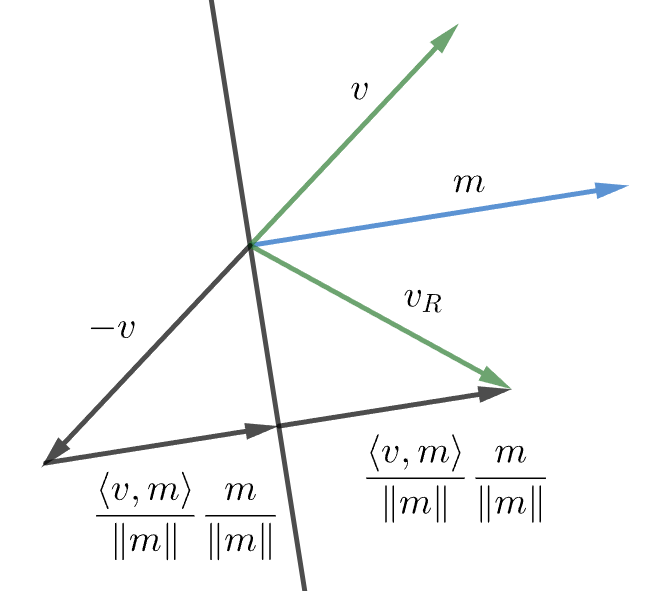
\includegraphics[width=0.4\textwidth]{chapters/theoretical_foundations/sections/non-eudlidean-spaces/resources/reflection.png}
    \caption{Reflection of $v$ on vector $m$}
    \label{fig:reflection}
\end{figure}
$$v_R = 2 \frac{\langle v, m \rangle}{\lVert m \rVert}\frac{m}{\lVert m \rVert} - v = 2\frac{\langle v, m\rangle}{\langle m,m\rangle}m - v.$$
It can be verified that this definition satisfies the intuitive conditions of a reflection:
\begin{itemize}
    \item The reflected vector $v_R$ lies in the plane spanned by $v$ and $m$,
    \item The transformation is an isometry, i.e. $\lVert u - v \rVert = \lVert u_R - v_R \rVert$.
\end{itemize}
We should also note that given a point $p$ in the geometry, i.e. satisfying $\langle p, p \rangle = \mathcal{L}$, its reflection, $p'$, is also in the geometry.

\subsubsection{Translation}
Just like in Euclidean space, we can define translation in terms of an even number of reflections.
More specifically, the translation will be defined by specifying two points: \textit{geometry origin}, $g = (0, 0, 0, 1)$ and \textit{translation target}, $q$, which is the point that the geometry origin is translated to.
Now we can define that the translation is the composition of two reflections: one on the vector $m_1 = g$ and the second one on the vector $m_2 = g + q$, which is halfway between $g$ and $q$.
Applying the first reflection to an arbitrary point $p$ gives a point
$$p' = 2 \frac{\langle p, g \rangle}{\langle g, g \rangle}g - p = 2p_w g - p,$$
and the second reflection applied to $p'$ yields a point
\begin{equation} \label{eq:translation}
    p'' = 2 \frac{\langle p', g + q \rangle}{\langle g + q, g + q \rangle}(g + q) - p'
    = 2 p_w q + p - \frac{p_w + \mathcal{L}\langle p, q \rangle}{1 + q_w}(g + q).
\end{equation}
The effect of applying translation to an arbitrary point $a$ is shown in \autoref{fig:translation}.\\
\begin{figure}[h]
    \centering
    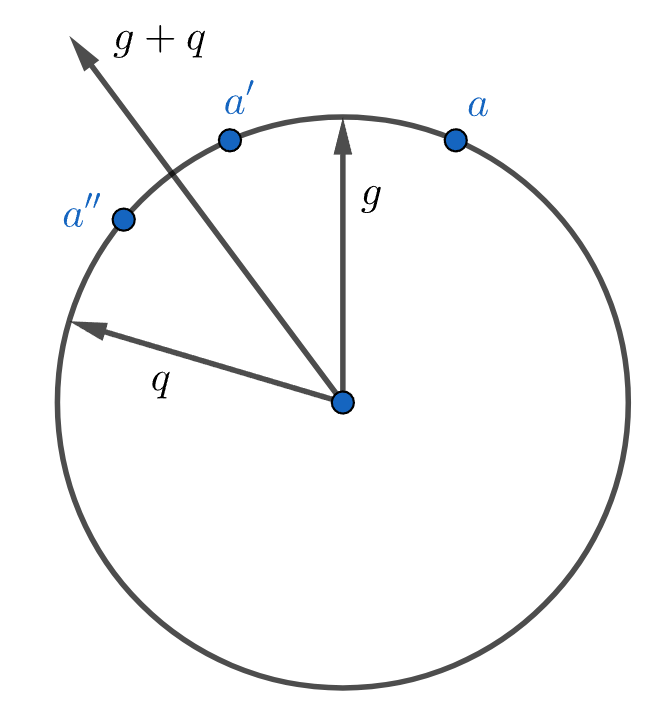
\includegraphics[width=0.4\textwidth]{chapters/theoretical_foundations/sections/non-eudlidean-spaces/resources/translation.png}
    \caption{Translation of a point $a$}
    \label{fig:translation}
\end{figure}
It can be verified that the geometry origin $g$ is indeed translated to point $g'' = q$.
We can evaluate the formula for the basis vectors $i = (1, 0, 0, 0)$, $j = (0, 1, 0, 0)$, $k = (0, 0, 1, 0)$, and $l = (0, 0, 0, 1)$ obtaining the translation matrix
\begin{equation} \label{eq:translation-matrix}
    T(q) = \begin{bmatrix}
        1 - \mathcal{L}\frac{q_x^2}{1 + q_w} & -\mathcal{L}\frac{q_x q_y}{1 + q_w}  & -\mathcal{L}\frac{q_x q_z}{1 + q_w}  & -\mathcal{L} q_x \\
        -\mathcal{L}\frac{q_y q_x}{1 + q_w}  & 1 - \mathcal{L}\frac{q_y^2}{1 + q_w} & -\mathcal{L}\frac{q_y q_z}{1 + q_w}  & -\mathcal{L} q_y \\
        -\mathcal{L}\frac{q_z q_x}{1 + q_w}  & -\mathcal{L}\frac{q_z q_y}{1 + q_w}  & 1 - \mathcal{L}\frac{q_z^2}{1 + q_w} & -\mathcal{L} q_z \\
        q_x                                  & q_y                                  & q_z                                  & q_w
    \end{bmatrix}
\end{equation}
It can be seen that the translation is an isometry since the row vectors of the matrix are orthonormal.

\subsubsection{Rotation}
It can be shown that a rotation about an axis through the origin is the same as the Euclidean rotation about the same axis \cite{Philips-Mark-Gunn1992}.

\subsubsection{Camera transformation}
% The camera transformation is defined in terms of the \textit{camera position} $e$, \textit{gaze direction} $g$, and the \textit{view-up vector} $t$.
% The camera position is a location that the camera "sees from", the gaze direction is a vector in the direction the camera is looking, and the view-up vector is a vector that points "to the sky".
% Using these vectors we can define the \textit{view space}, i.e. the camera's local coordinate system with the camera at the geometry origin and basis vectors $i'$, $j'$, and $k'$ defined as follows:
% \begin{equation*}
%     \begin{split}
%         k' = -\frac{g}{\lVert g \rVert}                    \\
%         i' = \frac{t \times k'}{\lVert t \times k' \rVert} \\
%         j' = k' \times i'
%     \end{split}
% \end{equation*}

The camera transformation allows us to describe the scene from the viewer's perspective.
The transformation is defined in terms of the \textit{eye position} $e$, and three orthonormal vectors in the tangent space of the eye:
\begin{enumerate}
    \item the right direction $i'$,
    \item the up direction $j'$, and
    \item the negative view direction $k'$.
\end{enumerate}
An example in \autoref{fig:tangent-space} shows the tangent space of the eye, with the $e$ vector marked green, $-k'$ marked blue, and $i'$ marked orange.\\
\begin{figure}[h]
    \centering
    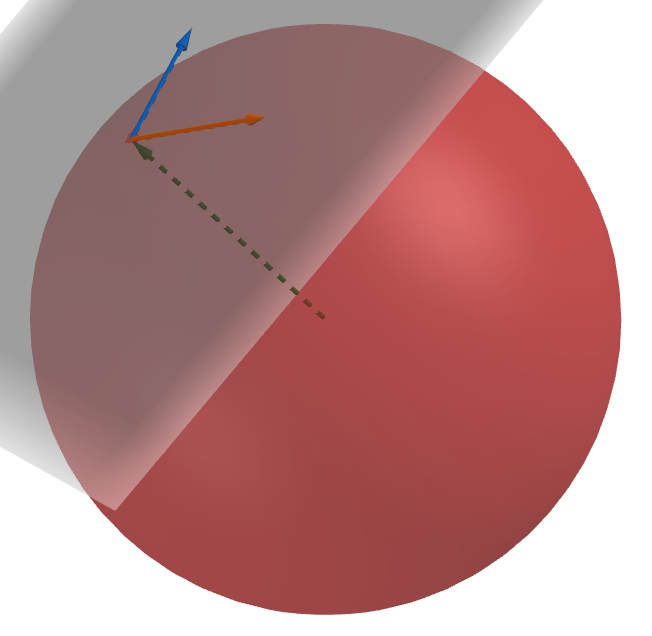
\includegraphics[width=0.4\textwidth]{chapters/theoretical_foundations/sections/non-eudlidean-spaces/resources/tangent-space.png}
    \caption{Tangent space of the camera}
    \label{fig:tangent-space}
\end{figure}
The transformation can be described by the matrix
\begin{equation} \label{eq:view-matrix}
    V =
    \begin{bmatrix}
        i'_x            & j'_x            & k'_x            & \mathcal{L}e_x \\
        i'_y            & j'_y            & k'_y            & \mathcal{L}e_y \\
        i'_z            & j'_z            & k'_z            & \mathcal{L}e_z \\
        \mathcal{L}i'_w & \mathcal{L}j'_w & \mathcal{L}l'_w & e_w
    \end{bmatrix}
\end{equation}
As the result of the transformation, the eye position is mapped to the geometry origin $g$.
Furthermore, the vectors $i'$, $j'$, and $k'$ are mapped to $i$, $j$, and $k$, respectively.

\subsubsection{Perspective transformation}
The perspective transformation is described using a projection matrix $P$.
The projection matrix we use in spherical geometry is identical to the one used in the \textit{Unity} implementation of \cite{Szirmay-Kalos2022} (see \url{https://github.com/mmagdics/noneuclideanunity}).
It is parameterized by the \textit{near plane distance} $n$, \textit{far plane distance} $f$, \textit{aspect ratio} ASP, and \textit{field of view} FOV:
\begin{equation*}
    P =
    \begin{bmatrix}
        s_x & 0   & 0  & 0  \\
        0   & s_y & 0  & 0  \\
        0   & 0   & 0  & -1 \\
        0   & 0   & -n & 0
    \end{bmatrix},
\end{equation*}
where $s_x = 2n / (r - l)$, $s_y = 2n / (t - b)$, and $r$, $l$, $t$, $b$ are defined in terms of $u = f \tan(\mathrm{FOV})$:
\begin{equation*}
    r = u \cdot \mathrm{ASP}, \,
    l = -u \cdot \mathrm{ASP}, \,
    t = u, \,
    b =  -u.
\end{equation*}
For hyperbolic and Euclidean geometries, the standard projection matrix is used.

\subsubsection*{Porting objects}
The positions of objects in the scene are specified in a 3-dimensional Euclidean space.
They are then "transported" or \textit{ported} to a non-Euclidean space of choice.
One possible mapping that could be used for this purpose is called the exponential map.
For a given point $p$ in the 3-dimensional Euclidean space with coordinates $(x, y, z)$ the mapping to elliptic geometry is given by
\begin{equation} \label{eq:elliptic-porting}
    \mathcal{P}_E(p) = (p / d \sin(d), \cos(d)),
\end{equation}
and for hyperbolic space, it is given by
\begin{equation*}
    \mathcal{P}_H(p) = (p / d \sinh(d), \cosh(d)),
\end{equation*}
where $d = \lVert p \rVert$.
The effect of porting a 1-dimensional point $p$ onto a 1-dimensional elliptic space can be seen in \autoref{fig:exp-map}.
\begin{figure}[h]
    \centering
    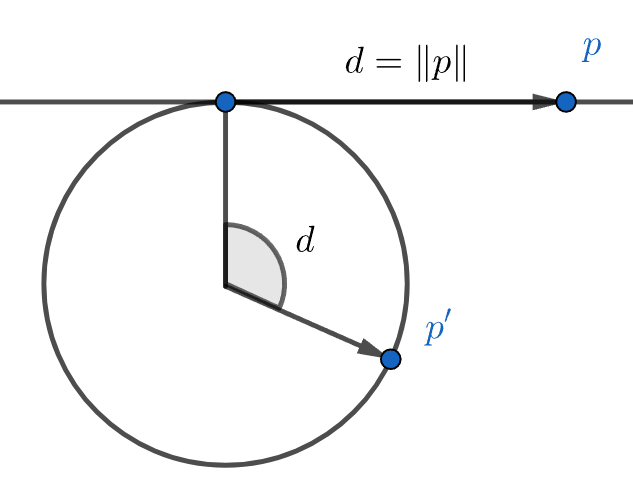
\includegraphics[width=0.4\textwidth]{chapters/theoretical_foundations/sections/non-eudlidean-spaces/resources/exp-map.png}
    \caption{Exponential map}
    \label{fig:exp-map}
\end{figure}

\subsubsection*{Porting vectors}
A vector $v$ starting at a point $p$ can be ported to non-Euclidean space by translating it to a point $\mathcal{P}(p)$.
Hence the ported vector $v'$ is given by
\begin{equation} \label{eq:porting-vector}
    v' = (v, 0) T(\mathcal{P}(p)),
\end{equation}
where $T$ is the translation matrix \ref{eq:translation-matrix}.